\documentclass[10pt,a4paper]{article}
\usepackage[utf8]{inputenc}
\usepackage[english]{babel}
\usepackage[T1]{fontenc}
\usepackage{amsmath}
\usepackage{amsfonts}
\usepackage{amssymb}
\usepackage{graphicx}
\usepackage{listings}
\author{Milan Tepic, Ivan Antunovic, Kareem Elzayat, Peter von Zameck Glyscinski}
\title{Assignment 3 Team 5}
\bibliographystyle{plain}

\begin{document}
\maketitle
\section*{Task 1}
\subsection*{a)}
\begin{figure}[h]
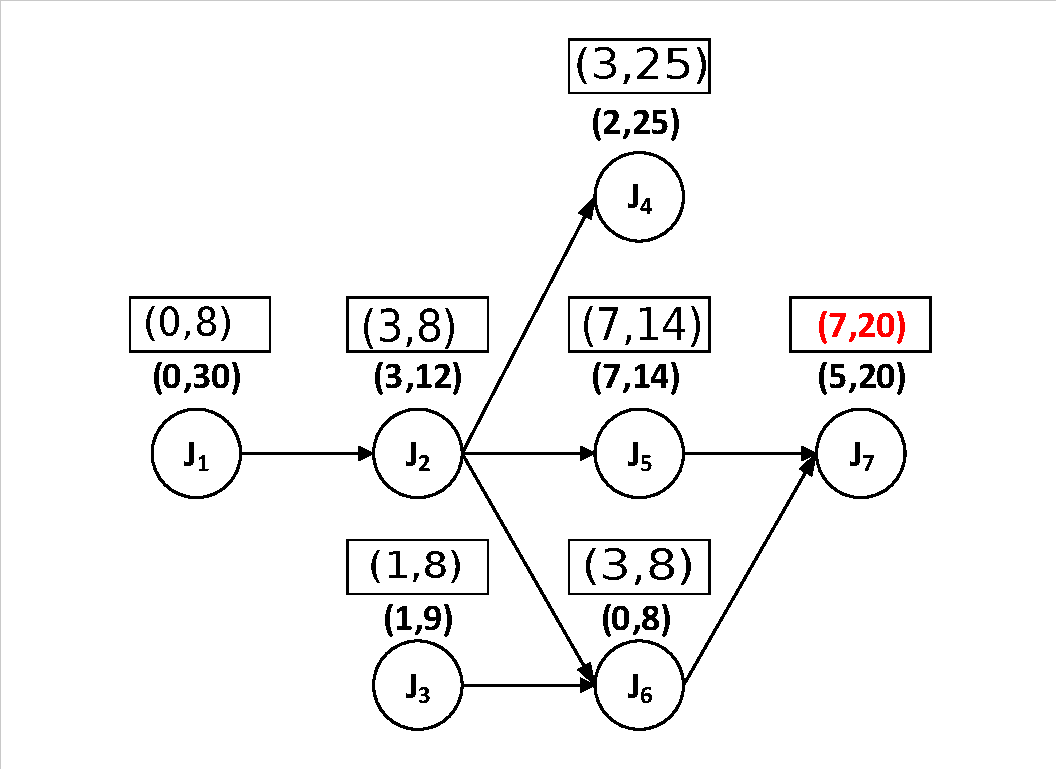
\includegraphics[width=\linewidth]{1a.pdf}
\caption{Effective Release time and Deadline.} 
\label{fig:1a}
\end{figure}
\newpage
\subsection*{b)}
\subsubsection*{i)}
The graph in figure \ref{fig:1bi} shows the network-flow graph with a feasible solution for the max-flow.
Edges are labeled with (flow|capacity).

\begin{figure}[h]
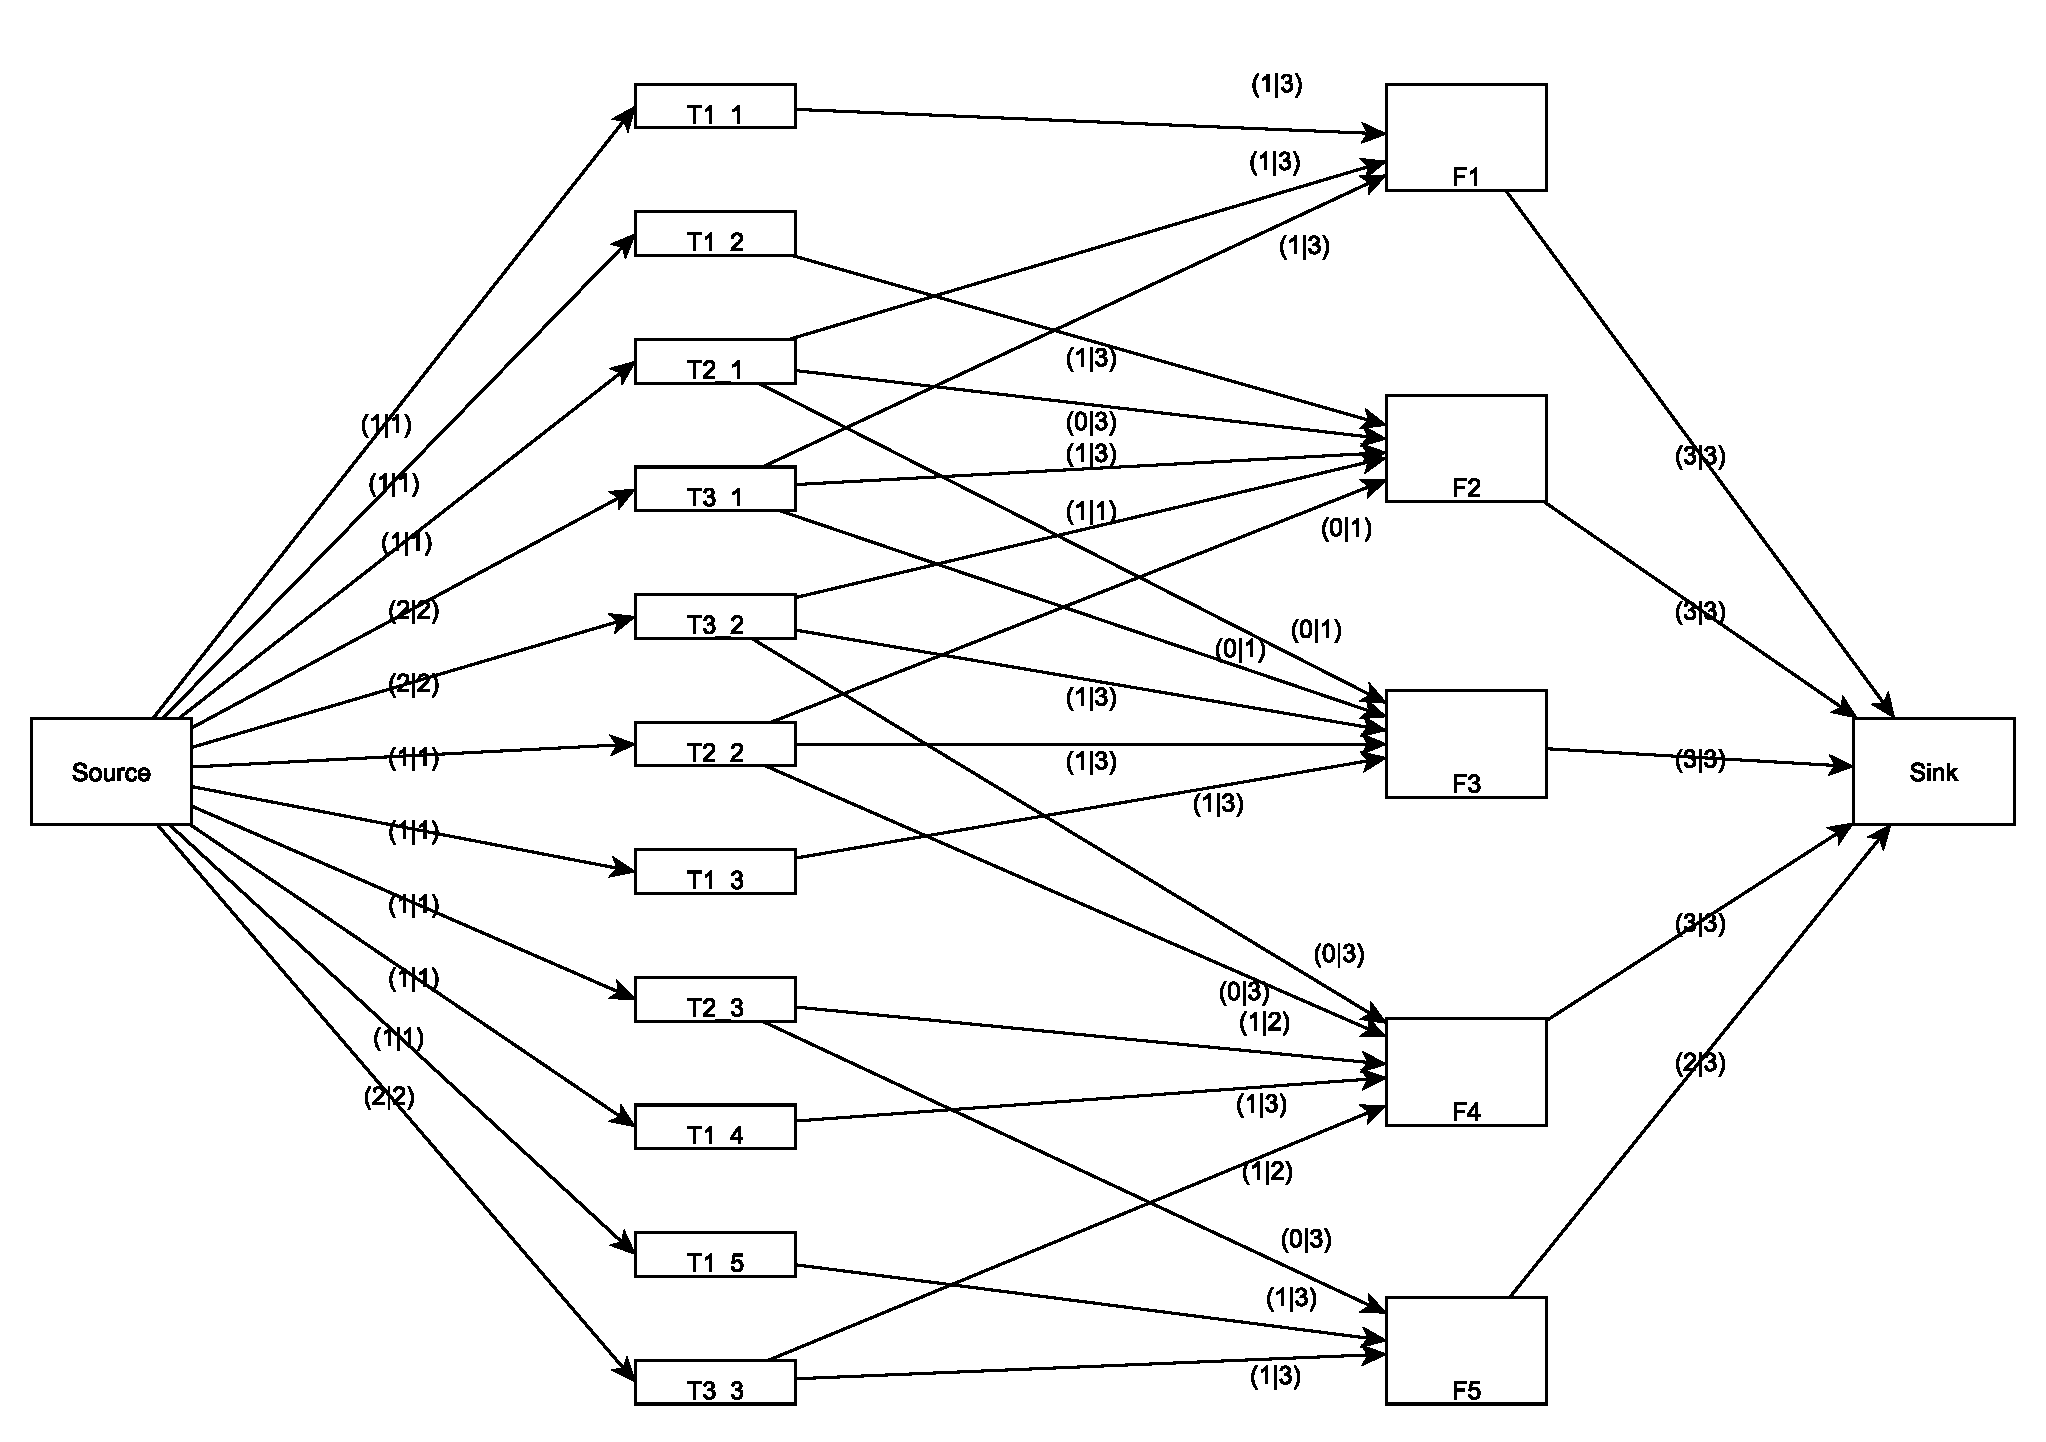
\includegraphics[width=\linewidth]{maxflow_1b.pdf}
\caption{Network flow graph for task 1 b) i).}
\label{fig:1bi}
\end{figure}

\begin{figure}[h]
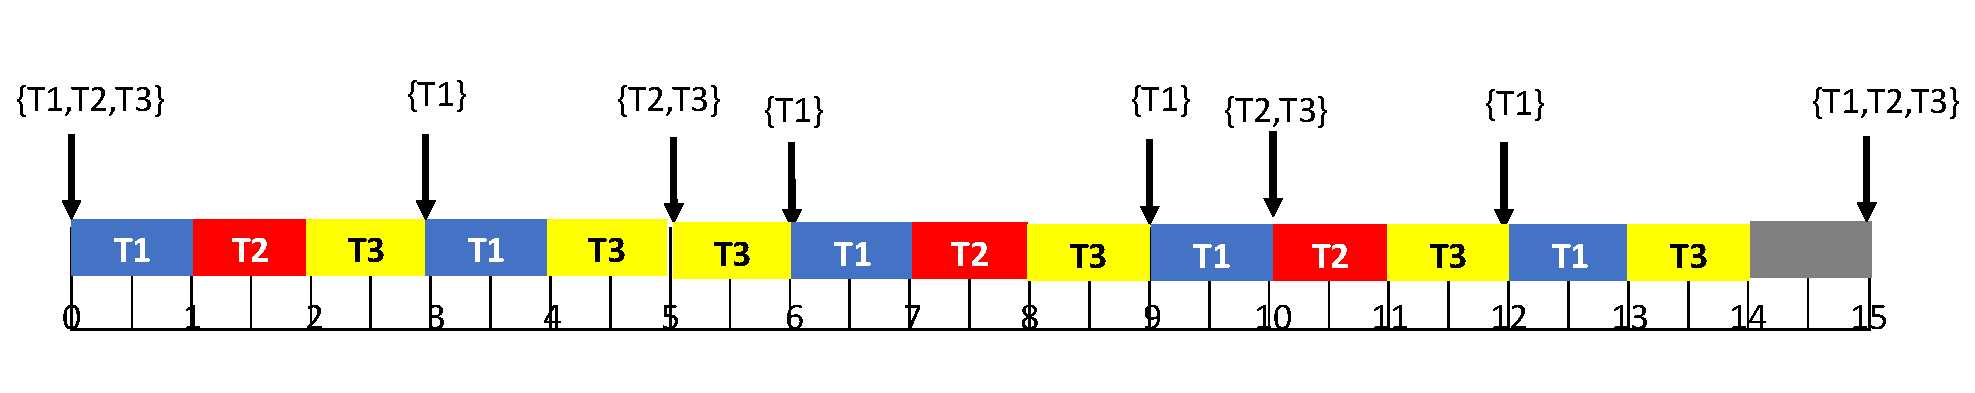
\includegraphics[width=\linewidth]{1b-timming-diagram.pdf}
\caption{Timming diagram for task 1 b) i).}
\label{fig:1biTimming}
\end{figure}

The resulting timming diagramm to the max-flow solution and also another proof that the task set is schedulable can be found in figure \ref{fig:1biTimming}.
\newpage
\section*{Task 2}
\subsection*{a)}

\begin{figure}[h]
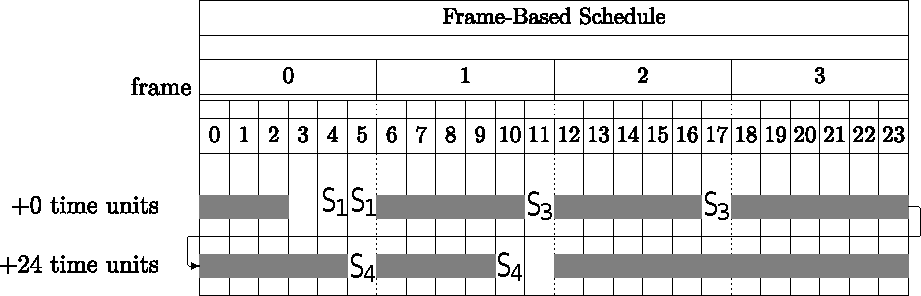
\includegraphics[width=\linewidth]{2a.pdf}
\label{fig:2a}
\end{figure}

\textbf{Note:} If sporadic task gets released within frame k, acceptance test can be only done at the beginning of the k+1 frame.

\subsection*{b)}
$U = \frac{27}{42} = 0.642$
\newline
$U_A = \frac{2.5}{31} + \frac{3.375}{45} + \frac{2.25}{54} + \frac{2.5}{32} = 0.275$
\newline
$W_0 = \frac{8.25}{62} + \frac{12.625}{90} + \frac{6}{108} + \frac{8}{64} = 0.45$
\newline
$\lambda = \frac{1}{31} + \frac{1}{45} + \frac{1}{54} + \frac{1}{32} = 0.104$
\newline
$T_{queing} = \frac{W_0}{(1-U)^2[1 - \frac{U_A}{1 - U}]} = \frac{0.45}{(1-0.642)^2[1 - \frac{0.275}{1 - 0.642}]} = 15.144$
\newline
$T_{average} = \frac{\frac{2.5}{31} + \frac{3.375}{45} + \frac{2.25}{54} + \frac{2.5}{32}}{\lambda(1 - U)} = \frac{0.275}{0.104(1 - 0.642)} = 7.398$
\newline
$W = T_{average} + T_{queing} = 7.398 + 15.144 = 22.542$
\section*{Task 3}
\subsection*{a)}
Check if task set $\mathbb{T}_1$ is RMA schedulable using utilization bound test \cite[~p27]{RTCLecture}:
\newline
$U = \frac{4}{15} + \frac{4}{20} + \frac{4}{30} + \frac{4}{60} = 0.67 \leq U_{RM}(4) = 4(2^{\frac{1}{4}} - 1) = 0.756$

\textbf{Conclusion:} The task set $T_1$ is RMA schedulable.

\subsection*{b)}
Check with Utilization bound test:
\newline
$U = \frac{4}{15} + \frac{4}{20} + \frac{8}{30} + \frac{8}{60} = 0.867 \nleq U_{RM}(4) = 4(2^{\frac{1}{4}} - 1) = 0.756$
Doesn't satisfy  utilization bound test.

Check with worst case simulation:
\newline
For task $A$: $4 \leq 15$
\newline
For task $B$: $C_B = (2 * 4) + 4 = 12 \leq 20$
\newline
For task $C$: $C_c = (2 * 4) + (2 * 4) + 8 = 24 \leq 30$
\newline
For task $D$: $C_d = (2 * 8) + (3 * 4) + (4 * 4) + 8 = 52 \leq 60$

\textbf{Conclusion:} The task set $T_2$ is RMA schedulable.

\subsection*{c)}
Since in current task set $\mathbb{T}_2$, task $A$ has the highest priority we want to choose $x$ such that task $D$ gets a smaller deadline. 
For that we choose $x=4$, resulting in a transformed task $D^\prime = (\frac{8}{4}, 60 - \frac{(4 - 1)60}{4}) = (2, 15)$. Since $p_{D} = p_{A}$ we assume that Pri(D) > Pri(A). With the new task $D^\prime$ we are able to schedule task set $T_2$ applying period transformation shown in figure \ref{fig:3c}.

\begin{figure}[!h]
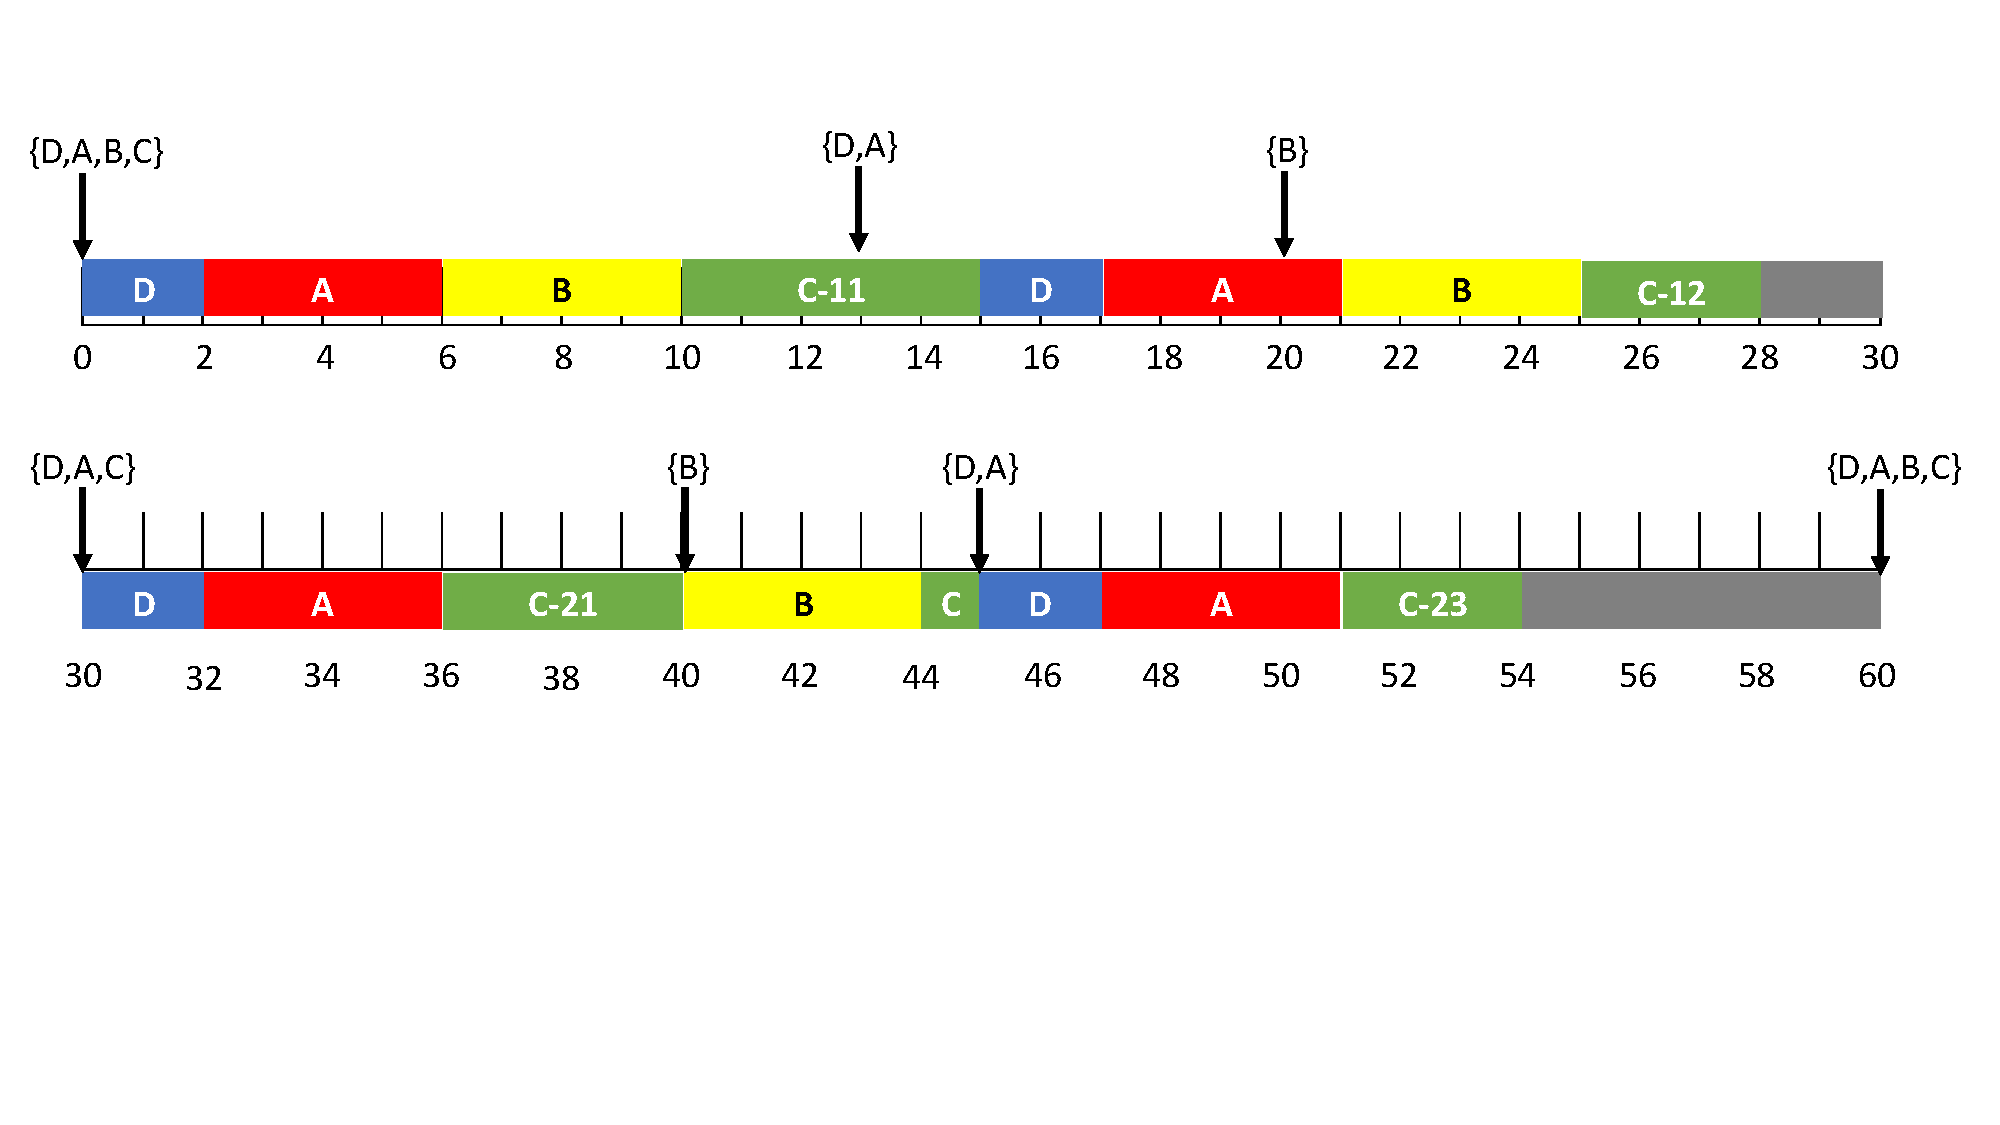
\includegraphics[width=\linewidth]{3c.pdf}
\caption{Timming diagram for task 3 c}
\label{fig:3c}
\end{figure}

\subsection*{d)}
Applying utilization bound test \cite[~p74]{RTCLecture}:\\

$\frac{e_A}{p_A} + \frac{e_B}{p_B} + \frac{e_C}{p_C} + \frac{e_D}{p_D} + max(\frac{b_C}{p_C}) \leq i($2^\frac{1}{i}-1)$ $  \newline

$\frac{4}{15} + \frac{4}{20} + \frac{8}{30} + \frac{8}{60} + max(\frac{4}{30}) = 1 \leq 4($2^\frac{1}{4}-1) = 0.76$ $ \newline

$1 \nleq 0.76$ 
\newline

Utilization bound test fails. Thus, we use generalized completion-time test using Time-demand analysis formula \cite[~p74]{RTCLecture}.

 \begin{enumerate}
    \item Task A: \newline
    $t_0$ = \sum_{i=1}^{1} $e_i$ = $e_A = 4 \leq d_A = 15$, task A is schedulable.
    
    \item Task B: \newline
    $t_0$ = \sum_{i=1}^{2} $e_i$ = $e_A$ + $e_B$ = 4 + 4 = 8 \\
    
    $t_1 = W_1(t_0)$ = $e_B + b_B$ + \sum_{k=1}^{1} $\lceil \frac{t_0}{p_k} \rceil\times e_k$ = $e_B + b_B$ + $\lceil \frac{t_0}{p_A} \rceil\times e_A = 4 + 0 + $\lceil \frac{8}{15} \rceil\times 4 = 8$ \newline
    
    Since $t_0 = t_1 = 8$ and $8 = t_1\leq d_B = 20$, task B is schedulable.

    \item Task C: \newline

     $t_0$ = \sum_{i=1}^{3} $e_i$ = $e_A + e_B + e_C$ = 4 + 4 + 8 = 16 \\
     
    $t_1 = W_1(t_0)$ = $e_C + b_C$ + \sum_{k=1}^{2} $\lceil \frac{t_0}{p_k} \rceil \times e_k$ = $e_B + b_B + \lceil \frac{t_0}{p_A} \rceil \times e_A + \lceil \frac{t_0}{p_B} \rceil \times e_B$ = 8 + 4 + $\lceil \frac{16}{15} \rceil\times 4 + 
    \lceil \frac{16}{20} \rceil\times 4 = 24$ \newline
    
    $t_2 = W_2(t_1)$ = $e_C + b_C$ + \sum_{k=1}^{2} $\lceil \frac{t_1}{p_k} \rceil\times e_k$ = $e_B + b_B$ + $\lceil \frac{t_1}{p_A} \rceil\times e_A + \lceil \frac{t_1}{p_B} \rceil \times e_B = 8 + 4 + \lceil \frac{24}{15} \rceil\times 4 + 
    \lceil \frac{24}{20} \rceil\times 4 = 24$ \newline
    
    Since $t_1 = t_2 = 24$ and $24 = t_2\leq d_C = 30$, task C is schedulable.
    
    
    
    \item Task D: \newline
    $t_0$ = \sum_{i=1}^{4} $e_i$ = $e_A + e_B + e_C + e_D$ = 4 + 4 + 8 + 8 = 24 \\
    
    $t_1 = W_1(t_0)$ = $e_D + b_D$ + \sum_{k=1}^{3} $\lceil \frac{t_0}{p_k} \rceil\times e_k$ = $e_D + b_D$ + $\lceil \frac{t_0}{p_A} \rceil\times e_A + \lceil \frac{t_0}{p_B} \rceil\times e_B + \lceil \frac{t_0}{p_C} \rceil\times e_C$ = 8 + 8 + $\lceil 
    \frac{24}{15} \rceil\times 4 
    + 
    \lceil \frac{24}{20} \rceil\times 4
    + 
    \lceil \frac{24}{30} \rceil\times 8 = 40$ \\
    
    $t_2 = W_2(t_1)$ = $e_D + b_D$ + \sum_{k=1}^{3} $\lceil \frac{t_1}{p_k} \rceil\times e_k$ = $e_D + b_D$ + $\lceil \frac{t_1}{p_A} \rceil\times e_A + \lceil \frac{t_1}{p_B} \rceil\times e_B + \lceil \frac{t_1}{p_C} \rceil\times e_C$ = 8 + 8 + $\lceil 
    \frac{40}{15} \rceil\times 4 
    + 
    \lceil \frac{40}{20} \rceil\times 4
    + 
    \lceil \frac{40}{30} \rceil\times 8 = 52$ \\
    
    $t_3 = W_3(t_2)$ = $e_D + b_D$ + \sum_{k=1}^{3} $\lceil \frac{t_2}{p_k} \rceil\times e_k$ = $e_D + b_D$ + $\lceil \frac{t_2}{p_A} \rceil\times e_A + \lceil \frac{t_2}{p_B} \rceil\times e_B + \lceil \frac{t_2}{p_C} \rceil\times e_C$ = 8 + 8 + $\lceil 
    \frac{52}{15} \rceil\times 4 
    + 
    \lceil \frac{52}{20} \rceil\times 4
    + 
    \lceil \frac{52}{30} \rceil\times 8 = 60$ \newline
    
    $t_4 = W_3(t_3)$ = $e_D + b_D$ + \sum_{k=1}^{3} $\lceil \frac{t_3}{p_k} \rceil\times e_k$ = $e_D + b_D$ + $\lceil \frac{t_3}{p_A} \rceil\times e_A + \lceil \frac{t_0}{p_B} \rceil\times e_B + \lceil \frac{t_3}{p_C} \rceil\times e_C$ = 8 + 8 + $\lceil 
    \frac{60}{15} \rceil\times 4 
    + 
    \lceil \frac{60}{20} \rceil\times 4
    + 
    \lceil \frac{60}{30} \rceil\times 8 = 60$ \newline
    
    
    Since $t_3 = t_4 = 60$ and $60 = t_3\leq d_D = 60$, task D is schedulable.
    
    \textbf{Conclusion:} task set
    $\mathbb{T}_3$ is RMA schedulable even with blocking.
    
  \end{enumerate}


\bibliography{bibl}
\end{document}
